\documentclass[12pt,a4paper]{article}

\usepackage{sbc-template}

\usepackage{graphicx,url}

\usepackage[brazilian]{babel}
\usepackage[utf8]{inputenc}
\usepackage[T1]{fontenc}
\usepackage{url}

%Força o local da tabela H
\usepackage{float}

%Criar Bookmark
\usepackage{hyperref}
\hypersetup{pdftex,colorlinks=true,allcolors=black}
\usepackage{hypcap}
%     
\sloppy

\title{Proposta de Desenvolvimento de um Software para Gerenciar\\  Banco de Sementes Crioulas}

\author{Daniel Leonardo de Souza Teixeira\inst{1}, Bruno Moraes Rocha\inst{2}, \\Flávio Ferreira Borges\inst{3} , Hildeu Ferreira Assunção \inst{4}}


\address{Curso de Ciência da Computação - Universidade Federal de Goias 
  (UFG)\\
  Caixa Postal 03 -- 75.801-615 --Jatai -- GO -- Brazil
\email {daniel.fnz@hotmail.com, rocha3runo@gmail.com ,
  flavio@ufg.br,hildeu@ufg.br}
}

\begin{document} 

\maketitle

\begin{abstract}
This paper reports the observation and analysis of the storage process and search for seeds
Creoles stored by the Núcleo de Estudos Pesquisa e Extensão em Agricultura Familiar (NEAF)
and proposes a software to manage the same.

\end{abstract}
     
\begin{resumo} 

Este artigo relata a observação e análise do processo de armazenagem e busca de sementes
crioulas mantidas pelo Núcleo de Estudos Pesquisa e Extensão em Agricultura Familiar (NEAF), bem como propõe um software para gerencia-lo.\\


\end{resumo}


\section{Introdução}

Na Regional Jataí da Universidade Federal de Goiás (UFG) funciona o Núcleo de Estudos Pesquisa e Extensão em Agricultura Familiar (NEAF) juntamente com o Centro Integrado de Agroecologia (CIAGRO), onde são desenvolvidas atividades de experimentação, validação e disponibilização participativa de tecnologias apropriadas à agricultura familiar. Nesta perspectiva, o NEAF tem como objetivos o desenvolvimento de pesquisas, ações de ensino e de extensão para oferecer aos agricultores interessados, as condições técnicas de suporte ao processo de produção orgânica, bem como a transição agroecológica. 

As experimentações em Agroecologia e Agricultura Familiar são realizadas como base no uso de variedades de sementes crioulas disponíveis no Banco de Sementes do NEAF, o qual possibilita aos agricultores realizarem empréstimos de diversos tipos de sementes. As sementes crioulas se diferenciam das demais, pois são sementes que não sofreram modificações genéticas e são conservadas pelas famílias de agricultores ao longo dos séculos, adaptadas às suas condições de solo e clima \cite{pelwing2008sementes}.

 O Banco de Sementes do NEAF ainda não conta com nenhum catálogo, planilha ou controle de estoque de sementes contidas no mesmo. A sua estrutura é composta por dois armários de ferro com divisórias. As divisórias separam os diversos tipos de sementes em recipientes. Cada recipiente é etiquetado de forma manuscrita, onde contém o nome da semente, data e local da colheita. Esse registro manuscrito pode ausentar informações importantes da colheita e dificultar a leitura de acordo com a caligrafia. Outro ponto interessante é que as divisórias não são etiquetadas, para encontrar uma determinada semente demanda um tempo razoavelmente grande. 

A digitalização destes dados facilitará o trabalho na procura das informações, organizando sistematicamente todos os dados, garantira a perpetuação dos dados por maior tempo, pois os dados registrados somente no papel estão sujeitos a serem facilmente perdido, pois com o tempo os papéis já se tornam ilegíveis, além de outros danos físicos que podem sofrer. Desta forma, percebeu-se à necessidade de organizar e guardar estes dados de forma que auxiliem melhor o trabalho com as sementes crioulas no NEAF.

Sendo assim, o objetivo deste trabalho é propor uma intervenção sobre o processo de armazenagem, visando diminuir o tempo gasto para encontrar uma determinada semente, bem como emissão de relatórios de quantidades de sementes e suas respectivas datas de validades. Para isso, será feito um levantamento dos requisitos necessários para o desenvolvimento de um {\it Software}, que auxilie a equipe do NEAF no processo de etiquetagem de recipientes, procura nas divisórias e emissão de relatórios de estoque. 

O controle de estoque e etiquetagem são importantes, pois possibilita à equipe listar todas as sementes cadastradas no banco de sementes, bem como informações do local onde foi colhida, data de colheita, quantidade e data de validade, assim quando vencidas,pode-se removê-las do armário desocupando espaço, além de padronizar as etiquetas, o {\it software} vai indicar em qual divisória o recipiente com a semente se encontra, facilitando a sua busca.



\section{Diagnóstico da Situação Problema}

Definimos que seria feita uma análise sobre o processo de armazenagem e busca no Banco de Sementes Crioulas do NEAF. Sendo assim, o primeiro passo, foi à observação assistemática para entender o processo de armazenamento de sementes, foi constatado a ausência de um sistema de controle de estoque e a forma de etiquetação das sementes não contém nenhum padrão. Em segundo momento, percebemos que o processo de busca por sementes  demanda um tempo razoavelmente grande.

Com a observação de todas as fases do processo de armazenamento de sementes, desde a separação das melhores sementes, a escolha do recipiente, a etiquetação do recipiente e a escolha da divisória para servir como local de armazenagem, notamos que a etiquetação dos recipientes é realizada de forma manuscrita, tornando-se o processo cansativo para a equipe do NEAF e dificultando estabelecer um padrão de etiquetas. A não padronização das etiquetas pode ocultar informações importantes como: nome da semente, data e local da colheita, além de dificultar a leitura de acordo com a caligrafia. 

Foi constatado que no processo de busca por determinada semente é preciso realizar uma busca de prateleira por prateleira até encontrar o recipiente desejado, demandando um tempo razoavelmente grande. Além da demanda de tempo pela busca, a falta de um sistema de controle de estoque cria situações em que a busca se torna perdida, pois ao procurar por uma determinada semente, ela pode ter se esgotado ou não conter as quantidades suficientes para empréstimo para os agricultores. O controle das sementes permitem obter informações básicas para gerenciar da melhor maneira as sementes armazenadas.

Outro problema constatado foi no momento da  armazenagem, como não há uma padronização ao armazenar as sementes, ao buscar por uma determinada semente, é necessário fazer uma busca por todos os recipientes, o que notamos ser uma tarefa exaustiva com grande demanda de tempo, o mesmo não iria ocorrer se as semente do mesmo gênero ficassem agrupadas.


\section{Proposta de Intervenção}
A partir dos problemas identificados, que são: tempo desperdiçado na busca de sementes  e etiquetação realizada de forma  manuscritamente. Será feita a proposta de desenvolvimento de um {\it Software} que realizará o controle de estoque e  impressão de etiquetas padronizadas.

Para executar a proposta de intervenção foi utilizada a modelagem por prototipação, pois segundo \cite{sommerville} com a prototipação possibilita demonstrar conceitos, levantar os requisitos básicos, experimentar opções de projeto, e em geral para conhecer o problema e suas possíveis soluções. Com isso, a proposta passou por três etapas básicas da modelagem por prototipação: 1-levantamento de requisitos; 2-identificação dos autores e suas interações; 3-criação de protótipos de telas e funcionalidades identificadas.

A primeira etapa foi identificar os requisitos básicos do sistema, ou seja, funções que o sistema deve
fornecer. De acordo com a observação assistemática realizada sobre os processos de armazenagem e busca de sementes,  com isso chegou-se aos seguintes requisitos funcionais apresentados na Tabela \ref{tab:requisitosFuncionalidades} e aos requisitos não funcionas descritos na Tabela \ref{tab:requisitosnaoFuncionalidades}.

\begin{table}[H]
\centering
\hspace{0.1cm}
\caption{\label{tab:requisitosFuncionalidades}Requisitos funcionais identificados.}
\begin{tabular}{c|l}

\hline%-&---------------------------------------------------------------------------------------------------------------------------------------\\
Código 	& Descrição 																\\ 
\hline%-&---------------------------------------------------------------------------------------------------------------------------------------\\
		& O usuário deve ser capaz de: realizar uma busca por palavra chave, como:	\\ 
RF01	& *Nome da Semente, *Categoria da Semente, *Data de Vencimento ou \\
		&*Local da Colheita.	
							\\ 
\hline%-&---------------------------------------------------------------------------------------------------------------------------------------\\
RF02	& O usuário deve ser capaz de: alterar ou remover a semente cadastrada\\ 
		&no banco de dados. \\				
\hline%-&---------------------------------------------------------------------------------------------------------------------------------------\\ 
RF03	& O resultado da busca deverá conter: Nome da semente, *Local da colheita, \\ 
		&Data da colheita, *Data de vencimento e  *Quantidade total.										\\ 
\hline%-&---------------------------------------------------------------------------------------------------------------------------------------\\
RF04 	& Os armários e suas prateleiras deverão ser rotúlados para que o 							\\
		&{\it Software} aponte a posição que se encontra a respectiva semente. \\
\hline%-&---------------------------------------------------------------------------------------------------------------------------------------\\
 		& O usuário deve ser capaz de Cadastrar a Semente, informando os seguintes \\
RF05	& campos obrigatórios: *Nome da Semente,*Local da Colheita,\\
		& *Data da Colheita,*Validade e *Quantidade. 									\\ 
\hline%-&---------------------------------------------------------------------------------------------------------------------------------------\\
		& O sistema deve ser capaz de prover a impressão de etiquetas para os \\
RF06 	&recipientes das sementes, onde o usuário deverá selecionar uma semente\\
		&previamente cadastrada e digitar a quantidade de etiquetas a serem impressas.\\  
\hline%-&---------------------------------------------------------------------------------------------------------------------------------------\\
RF07 	& O usuário deve ser capaz de: emitir um relatório de todas as sementes\\ 
		& cadastradas no banco de dados e identificar as sementes já vencidas.										\\ 
\hline%-&---------------------------------------------------------------------------------------------------------------------------------------\\
RF08 	& O usuário deve ser capaz de: emitir um relatório de todas as sementes\\ 
		& prestes a vencer ou já vencidas.\\ 
\hline%-&---------------------------------------------------------------------------------------------------------------------------------------
RF09 	& O sistema deve alertar ao usuário que determinada semente está \\
		&em falta ou com seu estoque baixo;	\\
\hline%-&---------------------------------------------------------------------------------------------------------------------------------------
RF10 	& O usuário deve ser capaz de: gerenciar os armários. Onde e possível  \\
		& adicionar novos armários ou removê-los;\\
\hline%-&---------------------------------------------------------------------------------------------------------------------------------------
RF11 	& O usuário deve ser capaz de: Cadastrar armário, informando  *Rótulo e\\
		&*Quantidade de Prateleiras.	\\
\hline%-&---------------------------------------------------------------------------------------------------------------------------------------

\end{tabular} 
\end{table} 


\begin{table}[H]
\centering
\caption{\label{tab:requisitosnaoFuncionalidades}Requisitos não funcionais identificados.}
\begin{tabular}{c|l}

\hline%-&---------------------------------------------------------------------------------------------------------------------------------------\\
Código 	& Descrição 																\\ 
\hline%-&---------------------------------------------------------------------------------------------------------------------------------------\\
RNF01	& O sistema deve ser de fácil manuseio, possibilitando o usuário aprender  	\\ 
		& a utilizar o mesmo com o tempo máximo de 30 minutos. 
\\ 
\hline%-&---------------------------------------------------------------------------------------------------------------------------------------\\
RNF02	& O sistema deve executar em qualquer plataforma. Ex: Linux, MAC e Windows. 				\\ 
\hline%-&---------------------------------------------------------------------------------------------------------------------------------------\\ 
RNF03	& O sistema deve carregar no máximo 20 sementes por página, \\ 
		&sendo que para visualizar os próximos 20 itens, o usuário deve acessar\\
		&a próxima tela.										\\ 
\hline%-&---------------------------------------------------------------------------------------------------------------------------------------\\
RNF04 	& Ao remover ou atualizar algum cadastro, deve-se instantaneamente 							\\
		&ser atualizado no banco de dados. 										\\ 
\hline%-&---------------------------------------------------------------------------------------------------------------------------------------\\
\end{tabular} 
\end{table} 

Com os requisitos elicitados, o próximo passo identificar os atores envolvidos. Para realizar essa identificação foi utilizada o Diagrama de Casos de usos, pois segundo \cite{sommerville2009} o diagrama é utilizado para identificar os autores envolvidos e todas as possíveis interações, além de identificar novos requisitos não elicitados anteriormente. O Diagrama de Casos de Uso é apresentado na Figura \ref {figura:User_Case}.

\begin{figure}[htpb]
\centering % para centralizarmos a figura
\includegraphics[width=16cm]{Figuras/UserCase.jpg} % leia abaixo
\caption{Diagrama de Casos de Uso do software para gerenciar o estoque.} 
\label{figura:User_Case}
\end{figure}

Para um melhor entendimento, antes de iniciar os casos de usos (UC1 e UC4, Figura \ref{figura:User_Case}) é obrigatório que o funcionário realize o cadastro de uma semente no banco de dados. Os casos de usos  {\it [UC1] Buscar Semente} e {\it [UC4] Emitir Relatório} serão mais especificados nas Tabelas \ref{tabela:UC1} e \ref{tabela:UC4} abaixo.


\begin{table}[H]
\caption{Especificação do fluxo de realizar uma busca do Caso de Uso "Buscar Semente".}
\centering
\label{tabela:UC1}
\begin{tabular}{|l|c|}
\hline 
{ \it UC01 - Buscar Semente} \\ 
\hline 
{\bf Breve descrição do caso de uso:} permite ao funcionário buscar uma determinada\\ semente no banco de dados \\
{\bf Atores:} funcionários do NEAF.\\
{\bf Casos de uso relacionados:}\\
• [UC02] Imprimir Etiquetas;\\
• [UC07] Visualizar Prateleira;\\\\
{\bf Pré-condições:}\\
• A semente deve estar previamente cadastrada.
\\\\
{\bf Fluxo básico:}\\
1. O funcionário inicia o caso de uso "[UC1] Buscar Semente".\\
2. O sistema solicita o preenchimento do campo de pesquisa.\\
3. O funcionário informa as palavras chaves e realiza a busca.\\
\\
{\bf Fluxos alternativos:}\\
{\bf • [FA01] Imprimir etiqueta da semente}\\
	1. Após realizar a busca, o funcionário seleciona a opção "[UC2] Imprimir Etiquetas";\\
	2. O sistema solicita a quantidade de etiquetas para impressão;\\
	3. O sistema gera as etiquetas e realiza uma pré-visualização das mesmas;\\
{\bf • [FA02] Visualizar local na prateleira}\\
1. Após realizar a busca,  o funcionário seleciona a opção "[UC7] Visualizar Prateleira";\\
2. O sistema apresenta uma imagem dos armários, indicando a prateleira onde \\ se encontra a semente pesquisada;\\ 
{\bf • [FA03] Remover Semente}\\
1. Após realizar a busca,  o funcionário seleciona a opção "Remover Semente";\\
2. O sistema exibe a mensagem "Deseja Realmente Remover a Semente?"\\
Se "Sim", deleta a semente do banco de dados, Se "não" fecha a mensagem; \\ 
{\bf • [FA03] Editar Semente}\\
1. Após realizar a busca,  o funcionário seleciona a opção "Editar Semente";\\
2. O funcionário pode alterar os seguintes campos: Nome da Semente,\\
Local da Colheita, Data de Validade e Quantidade;\\
3. Ao realizar as alterações o funcionário deve clicar em salvar, salvando as\\
alterações e retornando a página de busca.
\\\\
{\bf Exceções:}\\
 {\bf [E01] Funcionário não preencheu o campo obrigatório de busca.}\\
1. O sistema informa que o campo não foi preenchido.
\\\\
{\bf Pós-condições:}\\
• O sistema realiza uma busca completa em seu banco de dados e apresenta\\ o resultado da busca na tela.\\
\hline 
\end{tabular} 
\end{table} 


\begin{table}[]
\caption{Especificação do Caso de Uso "Emitir Relatorio".}
\label{tabela:UC4}
\begin{tabular}{|l|c|}
\hline 
{ \it UC04 - Emitir Relatório} \\ 
\hline 
{\bf Breve descrição do caso de uso:} permite ao funcionário listar todas as sementes\\ cadastradas no banco de dados, e sementes prestes a vencer. 
\\
{\bf Atores:} funcionários do NEAF.
\\
{\bf Casos de uso relacionados:}\\
• [UC02] Imprimir Etiquetas;\\
• [UC05] Sementes Prestes a vencer;\\
• [UC06] Todas Sementes;\\
• [UC07] Visualizar Prateleira;
\\
{\bf Pré-condições:}\\
• Deve conter pelo menos uma semente cadastrada.
\\
\\
{\bf Fluxo básico:}\\
1. O funcionário inicia o caso de usos "Emitir Relatório", e "Todas Sementes";\\
2. O sistema deve listar todas sementes cadastradas no banco de dados;\\
3. O ao clicar em "Imprimir Relatório", o sistema deve gerar um arquivo Portable\\ Document Format(PDF)
com todas as sementes e seus respectivos atributos.
\\
\\
{\bf Fluxos alternativos:}\\
{\bf • [FA01] Emitir Relatório de Sementes perto do vencimento}\\
1. O funcionário inicia os casos de usos "Emitir Relatório", e "Sementes Prestes a vencer";\\
2. O sistema deve listar todas sementes com seus prazos prestes a vencer;\\
3. Ao clicar em "Imprimir Relatório", o sistema deve gerar um arquivo Portable\\ 
Document Format(PDF).\\
{\bf • [FA02] Imprimir etiqueta da semente}\\
	1. Após emitir o relatório, o funcionário seleciona a opção "Imprimir Etiqueta";\\
	2. O sistema solicita a quantidade de etiquetas para impressão;\\
	3. O sistema gera as etiquetas e realiza uma pré-visualização das mesmas;\\
{\bf • [FA03] Visualizar local na prateleira}\\
1. O funcionário seleciona a opção "Visualizar Prateleira";\\
2. O sistema apresenta uma imagem dos armários, indicando a prateleira onde \\ se encontra a semente pesquisada;\\ 
{\bf • [FA04] Remover Semente}\\
1. O funcionário seleciona a opção "Remover Semente";\\
2. O sistema exibe a mensagem "Deseja Realmente Remover a Semente?"\\
Se "Sim", deleta a semente do banco de dados, Se "não" fecha a mensagem; \\ 
{\bf • [FA05] Editar Semente}\\
1. O funcionário seleciona a opção "Editar Semente";\\
2. O funcionário pode alterar os seguintes campos: Nome da Semente,\\
Local da Colheita, Data de Validade e Quantidade;\\
3. Ao realizar as alterações o funcionário deve clicar em salvar, salvando as\\
alterações e retornando a página de busca.
\\\\
{\bf Exceções:}\\
 {\bf [E01] Não contém sementes cadastradas no banco.}\\
1. O sistema informa que não e possível emitir o relatório.
\\\\
{\bf Pós-condições:}\\
• O sistema realiza uma busca completa em seu banco de dados e apresenta\\ o relatório na tela.\\
\hline 
\end{tabular} 
\end{table} 

Após o levantamento dos requisitos e a identificação dos atores envolvidos, passou-se a criação de protótipos de telas do {\it Software} proposto. Segundo \cite{sommerville} a prototipação apoia o processo de validação dos requisitos o qual permite revelar erros e omissões nos requisitos propostos.

A Figura 2 apresenta a tela de busca por palavra chave. O campo de busca atende o RF01, onde é possível realizar a busca por palavras chaves relacionadas com a sementes e a exibição do resultado atende o RF02 e RF03. A separação dos armários e prateleiras estão de acordo com o RF04, possibilitando apontar o local que se encontra a semente visualmente.

\begin{figure}[H]
\centering % para centralizarmos a figuras
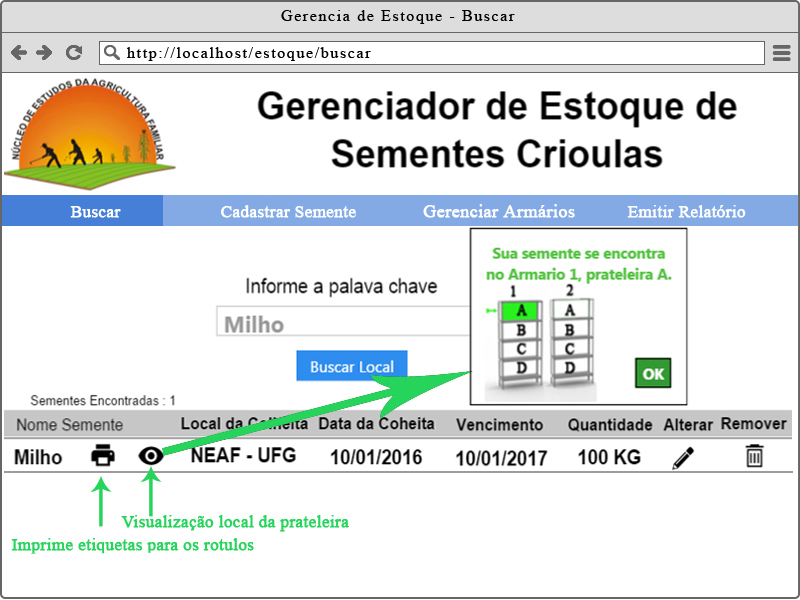
\includegraphics[width=14cm]{Figuras/busca.jpg} % leia abaixo
\label{figura:Tela_de_busca_sementes}
\caption{Tela de busca por semente.}
\end{figure}

Os campos necessários para realizar o cadastro como: Nome da Semente, Local da Colheita, Data de Colheita e sua Quantidade obedecem o RF05. Além de alertar o usuário quando algum campo preenchido de forma incorreta.
A Figura \ref{figura:Tela_cadastro} abaixo exibe a tela de cadastro de sementes.


\begin{figure}[H]
\centering % para centralizarmos a figura
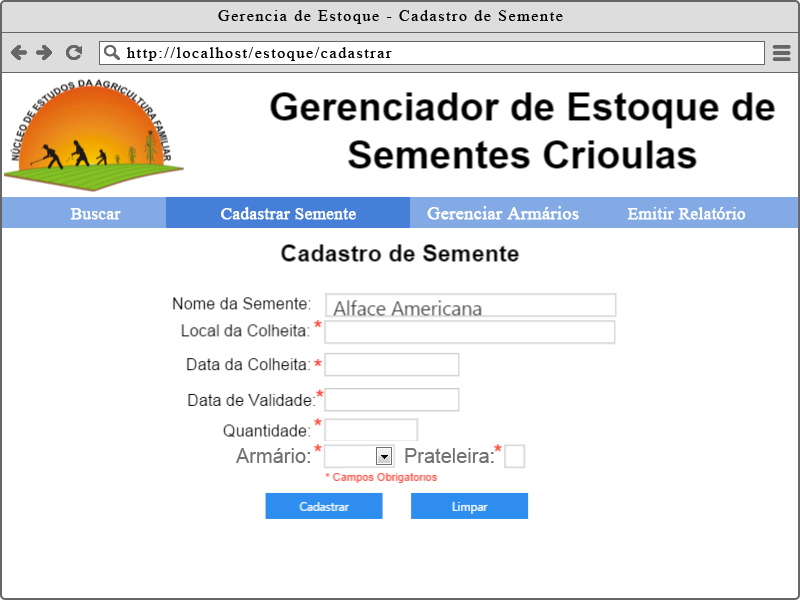
\includegraphics[width=14cm]{Figuras/cadastrar.jpg} % leia abaixo
\caption{Tela de cadastro de novas sementes.}
\label{figura:Tela_cadastro}
\end{figure}


\begin{figure}[H]
\centering % para centralizarmos a figura
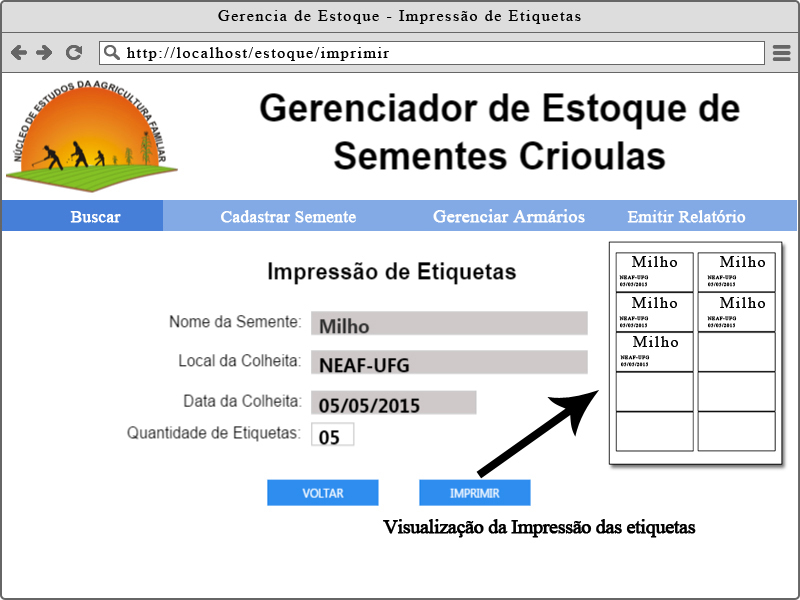
\includegraphics[width=14cm]{Figuras/imprimir.jpg} % leia abaixo
\caption{Tela de impressão de etiquetas para rotulos.}
\label{figura:Tela_impressao}
\end{figure}

Por outro lado a Figura \ref{figura:Tela_impressao} obedece o RF06, pois ilustra a tela de impressão de etiquetas. Deve-se realizar uma busca previamente pela semente cadastrada no banco e clicar no botão de impressão. Podemos observar a direita a visualização de impressão das etiquetas.


\begin{figure}[H]
\centering % para centralizarmos a figura
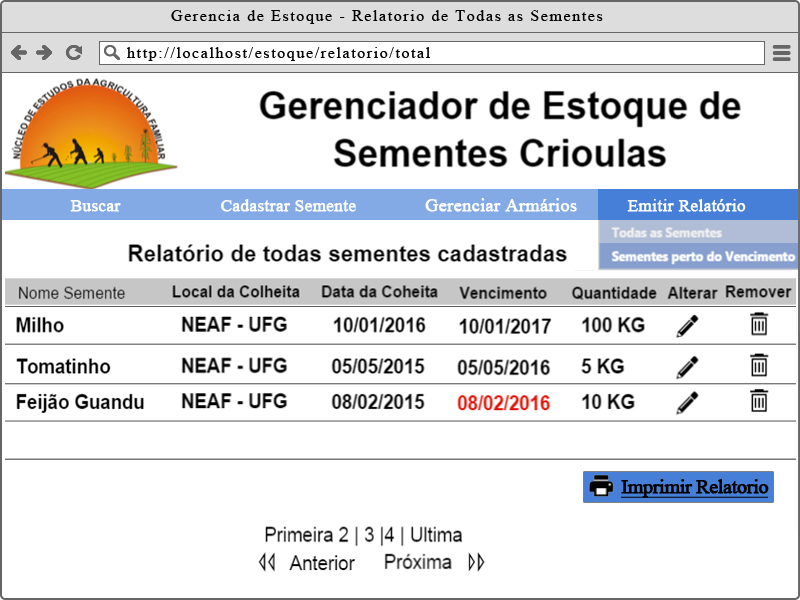
\includegraphics[width=14cm]{Figuras/relatorio_total.jpg} % leia abaixo
\caption{Tela de Geração de Relatório de Sementes Cadastradas.}
\label{figura:Tela_relatorio_total}
\end{figure}

Para a geração de relatório de todas as sementes cadastradas no banco, de acordo com o RF07 e RF09, a tela correspondente está sendo mostrada na Figura \ref{figura:Tela_relatorio_total}. Onde é possível visualizar e imprimir uma listagem de todas as sementes cadastradas no banco e seus respectivos atributos. Com esse relatório é possível alertar o usuário que o estoque de determinada semente está baixo, para que ele tome as possíveis soluções como: repor o estoque ou calcular se a quantidade  de sementes é o suficiente para o próximo plantio. Além de listar sementes vencidas para que sejam retiradas da prateleira, libera mais espaço de armazenamento. 

A Figura \ref{figura:Tela_relatorio_vencimento} apresenta a tela de emissão de relatório de sementes prestes a vencer ou já vencidas. Essa tela atende os RF04 e RF08 descritos acima. A partir desse relatório é possível determinar quais sementes irão vencer em breve, com isso possibilita uma forma mais adequada de utilizar as sementes antes do  seu prazo de vencimento. 

\begin{figure}[H]
\centering % para centralizarmos a figura
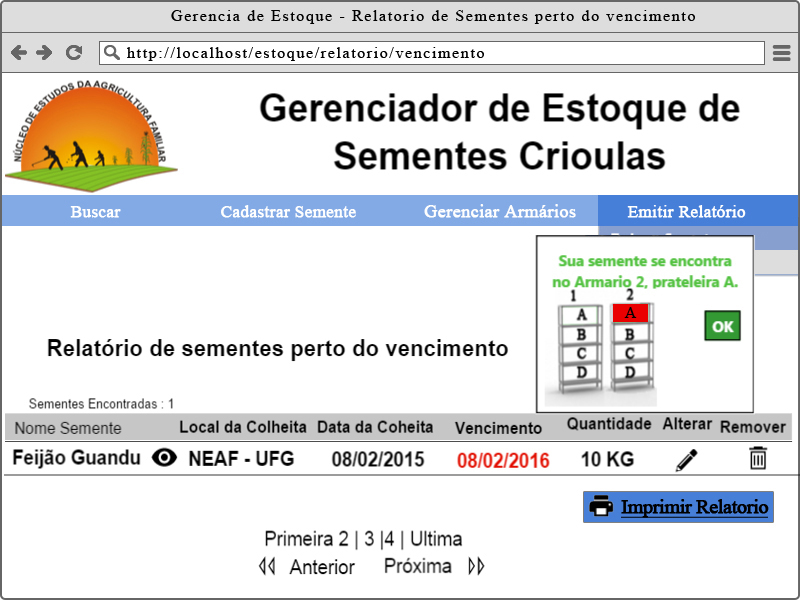
\includegraphics[width=14cm]{Figuras/relatorio_vencimento.jpg} % leia abaixo
\caption{Tela de emissão de relatorio com sementes perto do prazo de validade.}
\label{figura:Tela_relatorio_vencimento}
\end{figure}

\begin{figure}[H]
\centering % para centralizarmos a figura
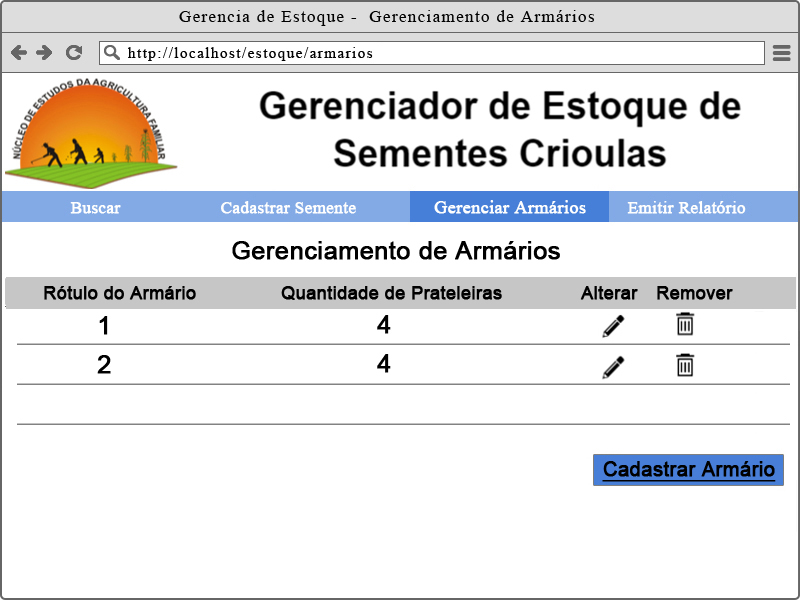
\includegraphics[width=14cm]{Figuras/gerenciar_armarios.jpg} % leia abaixo
\caption{Tela de gerenciamento de armários.}
\label{figura:Tela_gerencia_armario}
\end{figure}

\begin{figure}[H]
\centering % para centralizarmos a figura
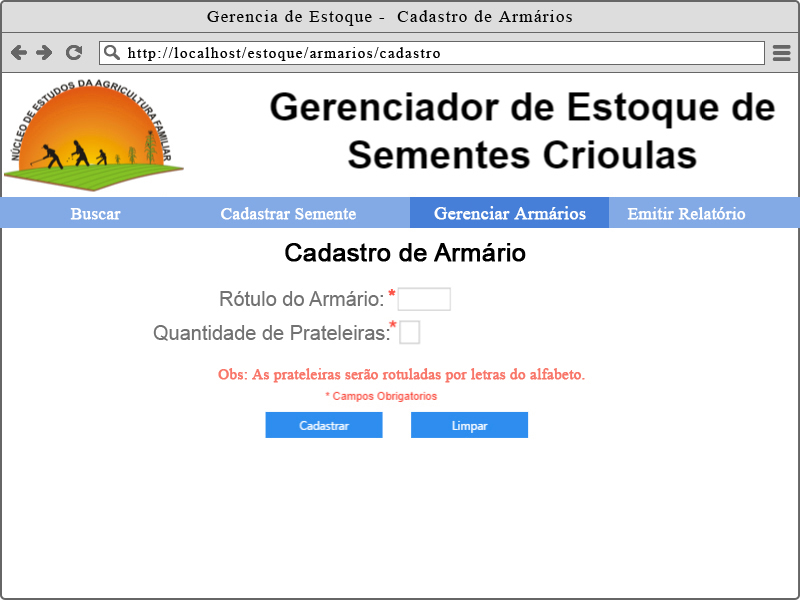
\includegraphics[width=14cm]{Figuras/cadastrararmario.jpg} % leia abaixo
\caption{Tela de cadastro de armário.}
\label{figura:Tela_cadastro_armario}
\end{figure}

A Figura \ref{figura:Tela_gerencia_armario} demonstra o gerenciamento de armários, atendendo os RF10, o qual possibilita adequar ao cotidiano se a demanda de armazenamento aumentar ou diminuir. A Figura \ref{figura:Tela_cadastro_armario} demonstra o cadastro de armário, o qual atende o RF11 e o caso de uso [UC9] Cadastrar Armário, possibilitando adicionar mais armários personalizados (a quantidade de prateleiras pode variar), de acordo com a necessidade de armazenar uma quantidade maior de sementes.

Como observado acima, os protótipos contemplam todos os requisitos levantados em fase inicial de projeto. O processo de prototipação facilita o entendimento dos requisitos, apresenta conceitos e funcionalidades do {\it Software} além de ser grande aliado ao desenvolvimento em curto prazo, adequado ao contexto da disciplina de Estágio Curricular Obrigatório.


\section{Planejamento da Avaliação da Proposta de Intervenção}

Para verificar se o {\it Software} proposto atenderá as necessidades aqui identificadas, foi utilizado um método de avaliação proposto por \cite{caldiera1994goal}, denominado GQM {\it (Goals-Questions-Metrics)}. O modelo de avaliação da proposta é apresentado abaixo.

{\bf• Objetivo:} analisar o {\it software} proposto visando avaliar sua eficácia quanto à minimização do tempo gasto com a busca de determinada semente e se as etiquetas padronizadas facilitam a leitura dos rótulos.\\\\
{\bf• Questões:}\\
{\bf  1}. O tempo gasto para encontrar uma determinada semente no banco diminuiu após a implantação do {\it Software}?\\
{\bf Métricas:} \\
{\bf  \#TGESA: } tempo gasto para encontrar uma determinada semente no banco antes da implantação do {\it Software};\\
{\bf  \#TGESD: } tempo gasto para encontrar uma determinada semente no banco depois da implantação do {\it Software};
\\
\\
{\bf   2}. A Padronização das etiquetas contribuiu para facilitar a leitura?\\
{\bf Métricas:} \\
{\bf  \#QUANTEA: } quantidade de vezes que a pessoa não conseguiu ler o rótulo antes da implantação do {\it Software};\\
{\bf  \#QUANTED: } quantidade de vezes que a pessoa não conseguiu ler o rótulo depois da implantação do {\it Software};\\
\\
{\bf• Interpretação das métricas:}\\
Se  \#TGESD < \#TGESA e \#QUANTED < \#QUANTEA, ambas com significância mínima acima de 95\%, pode-se afirmar que
o tempo de realização de busca e a taxa de erros ao ler um rótulo diminuíram, atingindo o objetivo da proposta.

\section{Relato das Atividades Desenvolvidas e Experiências Vivenciadas}
Devido a minha convivência anteriormente no Núcleo de Estudos Pesquisa e Extensão em Agricultura Familiar (NEAF) e a possibilidade de cursar a disciplina de Estágio Curricular Obrigatório, surgiu a oportunidade de apresentar uma proposta de intervenção sobre um problema presente no NEAF. Nesse sentido, foi usado a observação direta sobre o problema em questão.

Após feita a observação, deu-se inicio ao processo de desenvolvimento da proposta de intervenção que suprisse tal necessidade. Foi feita o levantamento de requisitos e a prototipação de prováveis telas do sistema.
As ferramentas utilizadas na proposta de intervenção foram a \cite{astah}, para criação dos diagramas da modelagem e a Balsamiq Mockups
\cite{balsamiq}, para a criação dos esboços das telas {\it software} proprietário que permite a
criação de esboços para diversos contextos e dispositivos).

A expêriencia de realizar o estágio foi satisfatória, pois além de colocar em prática as habilidades discutidas em sala de aula, foi  adiquirido
conhecimentos de que não são da área de Ciência da Computação. E a convivência com um grupo de pessoas de diversos cursos que são voluntários
no NEAF foi muito enriquecedora. 

A confecção do relatório e as telas do protótipo foram feitas por último, e contou-se com diversas revisões e refinamentos, até chegar ao presente documento.

\bibliographystyle{sbc}
\bibliography{referencias}

\end{document}
